% Provenance (never printed): cycle 3 "La planete Terre" and geography
% (weather and climate; reading a climate chart; the great climate zones of
% the world, hot, temperate and cold); see sources/book1/PROVENANCE.md.
% Book 1, grade 5, chapter 2.
\chapter{Weer en klimaat}\label{ch:g5:weather-and-climate}

In de tweede week van januari komen er twee ansichtkaarten aan op school.
Op de eerste, van Lena's nichtje, bouwen kinderen een zandkasteel op een
zonnig strand onder palmbomen. Op de tweede, van Toms oma, bouwen kinderen
een sneeuwpop in een besneeuwde tuin. ``Hoe kan het in dezelfde week zomer
en winter zijn?'' vraagt Tom.

Het is niet het \omterm{def:g1:watching-the-weather:weather}{weer} van één dag dat zo verschilt tussen die twee plaatsen.
Het is het \omterm{def:g1:watching-the-weather:weather}{weer} dat ze jaar na jaar hebben: hun \omterm{def:g5:weather-and-climate:climate}{klimaat}.

\begin{omfigure}
\begin{minipage}[b]{0.48\linewidth}\centering

\includegraphics[width=\linewidth]{images/book1/ai/g5-beach-postcard.jpg}
\end{minipage}\hfill
\begin{minipage}[b]{0.48\linewidth}\centering

\includegraphics[width=\linewidth]{images/book1/ai/g5-snowman-postcard.jpg}
\end{minipage}

{\small Twee ansichtkaarten uit dezelfde week van januari: een zonnig
strand en een besneeuwde tuin.}
\end{omfigure}

\begin{recall}
Het \omterm{def:g1:watching-the-weather:weather}{weer} is de toestand van de lucht op een bepaalde plaats en een bepaald
moment: zonnig, bewolkt, regenachtig, sneeuwachtig, winderig
(\cref{ch:g1:watching-the-weather}). Een thermometer meet de temperatuur
van de lucht, in graden Celsius; een \omterm{def:g4:clouds-rain-snow:rain-gauge}{regenmeter} meet de \omterm{def:g4:clouds-rain-snow:precipitation}{regen}, in
millimeter (\cref{ch:g4:clouds-rain-snow}). De \omterm{def:g3:continents-and-oceans:equator}{evenaar} loopt rond het
midden van de \omterm{def:g3:continents-and-oceans:globe}{globe}, halverwege tussen de \omterm{def:g3:continents-and-oceans:poles}{Noordpool} en de \omterm{def:g3:continents-and-oceans:poles}{Zuidpool}
(\cref{ch:g3:continents-and-oceans}). De natuurkundeboeken lieten zien dat
de Aarde in één jaar rond de Zon draait, en dat haar seizoenen komen door
de schuine stand van haar as: in de zomer klimt de Zon hoger aan de hemel
en zijn de dagen langer.
\end{recall}

\section{Weer is vandaag, klimaat is het gewone}

Het \omterm{def:g1:watching-the-weather:weather}{weer} verandert van dag tot dag, en zelfs van uur tot uur. \omterm{def:g5:weather-and-climate:climate}{Klimaat} is
iets anders.

\begin{definition}[Klimaat]\label{def:g5:weather-and-climate:climate}
Het \emph{klimaat}\index{klimaat} van een plaats is het \omterm{def:g1:watching-the-weather:weather}{weer} dat die
gewoonlijk heeft, maand na maand, over veel jaren: hoe warm of koud, hoe
nat of droog elk seizoen is. Weerkundigen berekenen het door het gemiddelde
te nemen van de metingen van 30 jaar.
% ledger: wmo:normal-30yr
\end{definition}

``Het regent vanochtend'' is een zin over het \omterm{def:g1:watching-the-weather:weather}{weer}. ``Hier regent het veel
in de herfst'' is een zin over het \omterm{def:g5:weather-and-climate:climate}{klimaat}. Eén koude dag in de zomer
verandert het \omterm{def:g5:weather-and-climate:climate}{klimaat} niet; het is gewoon ongewoon weer.

Weerkundigen over de hele wereld gebruiken dezelfde regel: ze nemen het
gemiddelde van 30 jaar metingen. De gemiddelden die nu worden gebruikt,
zijn die van de jaren 1991 tot 2020.
% ledger: wmo:normal-30yr

\section{Het klimaatdiagram}

Om het \omterm{def:g5:weather-and-climate:climate}{klimaat} van een plaats in één plaatje te laten zien, tekenen we een
diagram.

\begin{definition}[Klimaatdiagram]\label{def:g5:weather-and-climate:climate-chart}
Een \emph{klimaatdiagram}\index{klimaatdiagram} laat voor elke maand van het
jaar de gemiddelde temperatuur van een plaats zien (een lijn) en de
gemiddelde hoeveelheid \omterm{def:g4:clouds-rain-snow:precipitation}{regen} en \omterm{def:g4:clouds-rain-snow:precipitation}{sneeuw} die er valt (staven, in millimeter
water).
\end{definition}

\begin{omfigure}
\begin{tikzpicture}
  \begin{axis}[name=pax, width=0.55\linewidth, height=5.6cm, ymin=0, ymax=400,
      axis y line*=right, axis x line=none, ybar, bar width=7pt,
      ytick={0,100,...,400}, ylabel={regen (mm)}, xmin=0.4, xmax=12.6,
      tick label style={font=\scriptsize}, label style={font=\scriptsize},
      ylabel style={blue!60!black}]
    \addplot[fill=blue!40, draw=blue!60!black]
      table[x=month, y=prcp_mm] {figdata/out/grade-5-climate_charts-seattle.dat};
  \end{axis}
  \begin{axis}[width=0.55\linewidth, height=5.6cm, ymin=-30, ymax=40,
      axis y line*=left, axis x line*=bottom, xmin=0.4, xmax=12.6,
      xtick={1,...,12}, xticklabels={J,F,M,A,M,J,J,A,S,O,N,D},
      ytick={-30,-20,...,40}, ylabel={temperatuur ($^\circ$C)},
      tick label style={font=\scriptsize}, label style={font=\scriptsize},
      ylabel style={red!70!black}]
    \addplot[red!70!black, thick, mark=*, mark size=1.3pt]
      table[x=month, y=tavg_C] {figdata/out/grade-5-climate_charts-seattle.dat};
    \draw[gray!60] (axis cs:0.4,0) -- (axis cs:12.6,0);
    \begin{scope}[every node/.style={circle, draw, fill=white, inner sep=0.8pt,
        font=\scriptsize\bfseries}]
      \node[text=red!70!black, draw=red!70!black] at (axis cs:5.5,27) {1};
      \node[text=blue!60!black, draw=blue!60!black] at (axis cs:7,-19) {2};
    \end{scope}
  \end{axis}
  \node[anchor=north west, font=\scriptsize, align=left, text width=4.2cm]
    at ($(pax.outer north east)+(0.3,-0.1)$) {%
    \textcolor{red!70!black}{\textbf{1} De rode lijn: de gemiddelde temperatuur
    van elke maand, af te lezen op de linkerschaal.}\par\smallskip
    \textcolor{blue!60!black}{\textbf{2} De blauwe staven: de gemiddelde regen van
    elke maand, af te lezen op de rechterschaal.}\par\smallskip
    \textbf{3} De letters onder het diagram: de maanden, januari tot
    december.};
\end{tikzpicture}

{\small Het \omterm{def:g5:weather-and-climate:climate-chart}{klimaatdiagram} van Seattle, een stad aan de westkust van de
Verenigde Staten. Gemiddelden van de jaren 1991 tot 2020 (gegevens: NOAA).}
% ledger: data:b1-noaa-normals
\end{omfigure}

\begin{method}[Een klimaatdiagram lezen]\label{met:g5:weather-and-climate:reading}
\begin{enumerate}
  \item Zoek op de rode lijn de warmste en de koudste maand, en lees hun
        temperaturen af op de linkerschaal. Is de lijn vlak (het hele jaar
        dezelfde temperatuur) of gaat ze op en neer (warme en koude
        seizoenen)? Komt ze onder 0~$^\circ$C (vorst)?
  \item Zoek bij de blauwe staven de natste en de droogste maand, en lees
        ze af op de rechterschaal. Zijn de staven hoog of laag? Is er een
        droog seizoen?
  \item Vat het samen in één zin: ``het hele jaar heet en droog'', ``zacht
        en nat, met een droge zomer''{\ldots}
\end{enumerate}
\end{method}

\begin{example}[Seattle]\label{ex:g5:weather-and-climate:seattle}
In Seattle is augustus de warmste maand (ongeveer 20~$^\circ$C) en december
de koudste (ongeveer 6~$^\circ$C): de lijn gaat op en neer, maar komt nooit
onder het vriespunt. De hoogste staaf is die van november (ongeveer
160~mm), de laagste die van juli (ongeveer 15~mm). In één zin: zachte
winters, koele zomers, nat in de herfst en de winter, vrij droog in de
zomer. In een heel jaar valt er ongeveer 1\,000~millimeter \omterm{def:g4:clouds-rain-snow:precipitation}{regen}: een meter
water.
% ledger: data:b1-noaa-normals
\end{example}

\section{Vier klimaten}

Hier zijn de \omterm{def:g5:weather-and-climate:climate-chart}{klimaatdiagrammen} van vier plaatsen in de Verenigde Staten,
ver uit elkaar: Phoenix, in de \omterm{def:g5:weather-and-climate:desert}{woestijn} van Arizona; Hilo, op het eiland
Hawaï midden in de Stille \omterm{def:g2:water-on-earth:ocean}{Oceaan}; Seattle, aan de westkust; en Utqiaġvik,
in het hoge noorden van Alaska, aan de \omterm{def:g1:landscapes-around-us:water}{kust} van de Noordelijke IJszee. Alle
vier de diagrammen gebruiken dezelfde schalen, dus we kunnen ze in één
oogopslag vergelijken.

\begin{omfigure}
\def\gfivechart#1#2{%
\begin{tikzpicture}
  \begin{axis}[width=0.5\linewidth, height=4.6cm, ymin=0, ymax=400,
      axis y line*=right, axis x line=none, ybar, bar width=4pt,
      ytick={0,100,...,400}, xmin=0.4, xmax=12.6,
      tick label style={font=\tiny}]
    \addplot[fill=blue!40, draw=blue!60!black]
      table[x=month, y=prcp_mm] {figdata/out/grade-5-climate_charts-#1.dat};
  \end{axis}
  \begin{axis}[width=0.5\linewidth, height=4.6cm, ymin=-30, ymax=40,
      axis y line*=left, axis x line*=bottom, xmin=0.4, xmax=12.6,
      xtick={1,...,12}, xticklabels={J,F,M,A,M,J,J,A,S,O,N,D},
      ytick={-30,-20,...,40}, tick label style={font=\tiny},
      title={#2}, title style={font=\scriptsize\bfseries, yshift=-4pt}]
    \addplot[red!70!black, thick, mark=*, mark size=1pt]
      table[x=month, y=tavg_C] {figdata/out/grade-5-climate_charts-#1.dat};
    \draw[gray!60] (axis cs:0.4,0) -- (axis cs:12.6,0);
  \end{axis}
\end{tikzpicture}}%
\gfivechart{phoenix}{Phoenix: een hete \omterm{def:g5:weather-and-climate:desert}{woestijn}}\hfill
\gfivechart{hilo}{Hilo: een regenwoudklimaat}

\medskip
\gfivechart{seattle}{Seattle: een gematigd \omterm{def:g5:weather-and-climate:climate}{klimaat}}\hfill
\gfivechart{utqiagvik}{Utqiaġvik: een poolklimaat}

{\small Vier \omterm{def:g5:weather-and-climate:climate-chart}{klimaatdiagrammen} met dezelfde schalen: temperatuur in
$^\circ$C links (rode lijn), \omterm{def:g4:clouds-rain-snow:precipitation}{regen} in millimeter rechts (blauwe staven).
Gemiddelden van de jaren 1991 tot 2020 (gegevens: NOAA).}
% ledger: data:b1-noaa-normals
\end{omfigure}

\paragraph{De woestijn.} In Phoenix zijn de staven zo laag dat we ze
nauwelijks zien: in een heel jaar valt er minder dan 200 millimeter \omterm{def:g4:clouds-rain-snow:precipitation}{regen}.
De zomers zijn erg heet: in juli is de gemiddelde temperatuur 35 graden.
% ledger: data:b1-noaa-normals

\begin{definition}[Woestijn]\label{def:g5:weather-and-climate:desert}
Een \emph{woestijn}\index{woestijn} is een plaats waar heel weinig \omterm{def:g4:clouds-rain-snow:precipitation}{regen}
valt: minder dan 250 millimeter per jaar. Er kunnen weinig planten leven,
en de grond is vaak kaal.
% ledger: usgs:arid-250mm
\end{definition}

\omterm{def:g5:weather-and-climate:desert}{Woestijnen} zijn niet altijd heet. Kijk naar Utqiaġvik: daar valt minder dan
150 millimeter per jaar, nog minder dan in Phoenix: het is een koude
\omterm{def:g5:weather-and-climate:desert}{woestijn}. \omterm{def:g5:weather-and-climate:desert}{Woestijnen} kunnen heet of koud zijn.
% ledger: data:b1-noaa-normals, usgs:arid-250mm

\paragraph{Het regenwoud.} Hilo is het tegenovergestelde van Phoenix. Zijn
staven zijn de hoogste van de vier diagrammen: er valt meer dan
3\,000 millimeter \omterm{def:g4:clouds-rain-snow:precipitation}{regen} per jaar, en elke maand is nat. En zijn rode lijn
is bijna vlak: het hele jaar tussen 22 en 25 graden. Er is helemaal geen
winter.
% ledger: data:b1-noaa-normals

\begin{definition}[Regenwoud]\label{def:g5:weather-and-climate:rainforest}
Een \emph{regenwoud}\index{regenwoud} is een dicht bos van heel hoge bomen
dat groeit waar het het hele jaar door warm en nat is, met veel \omterm{def:g4:clouds-rain-snow:precipitation}{regen} in
elke maand. De meeste regenwouden liggen dicht bij de \omterm{def:g3:continents-and-oceans:equator}{evenaar}.
\end{definition}

\begin{omfigure}
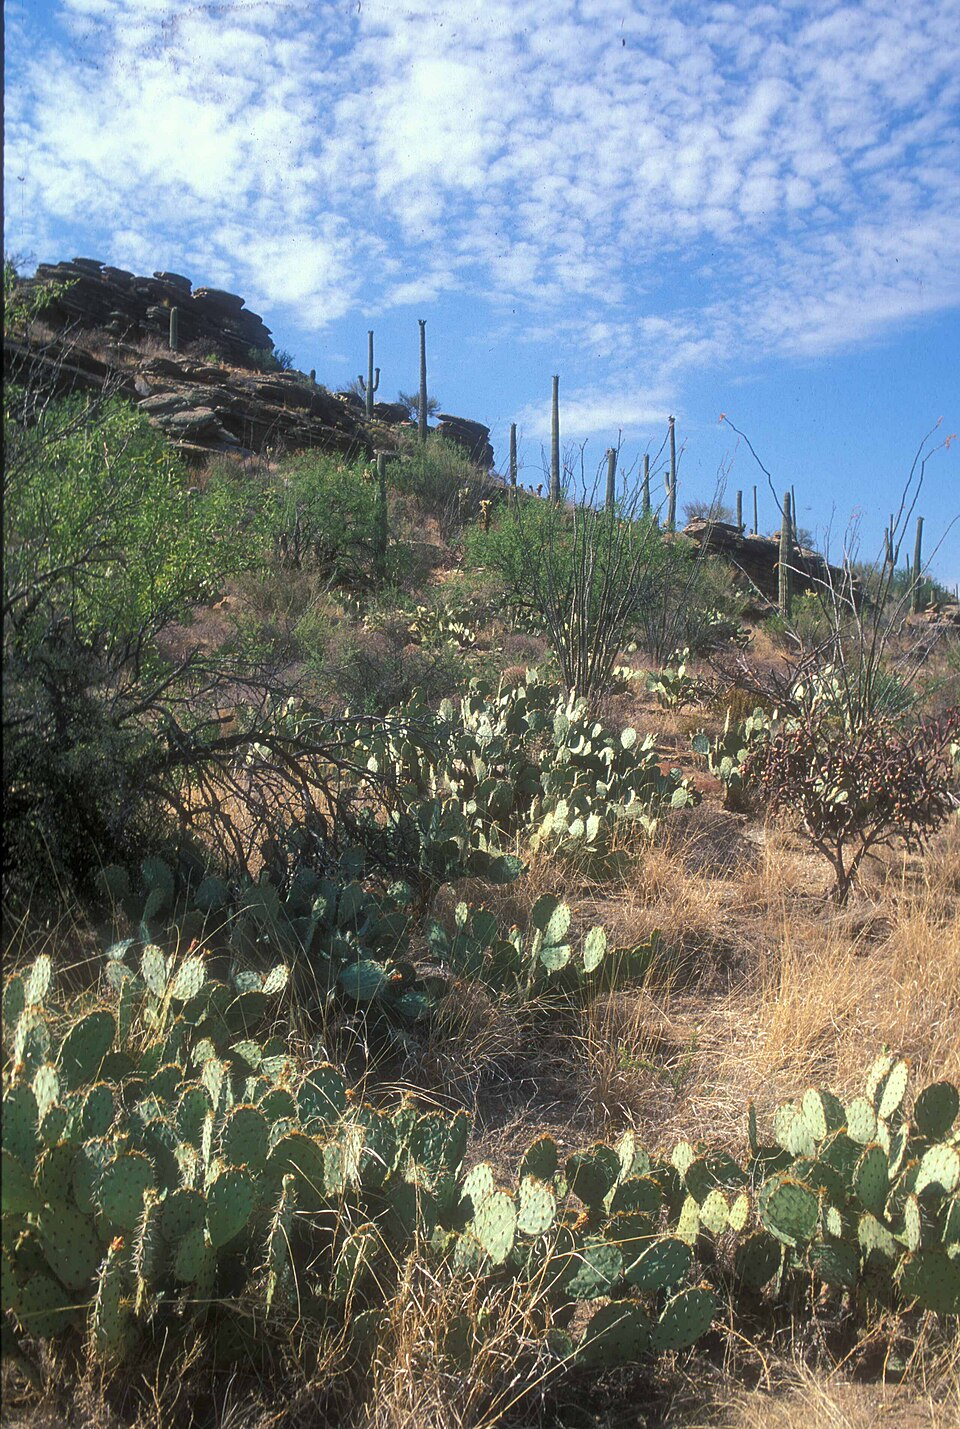
\includegraphics[height=3.6cm]{images/book1/g5-sonoran-desert.jpg}\quad
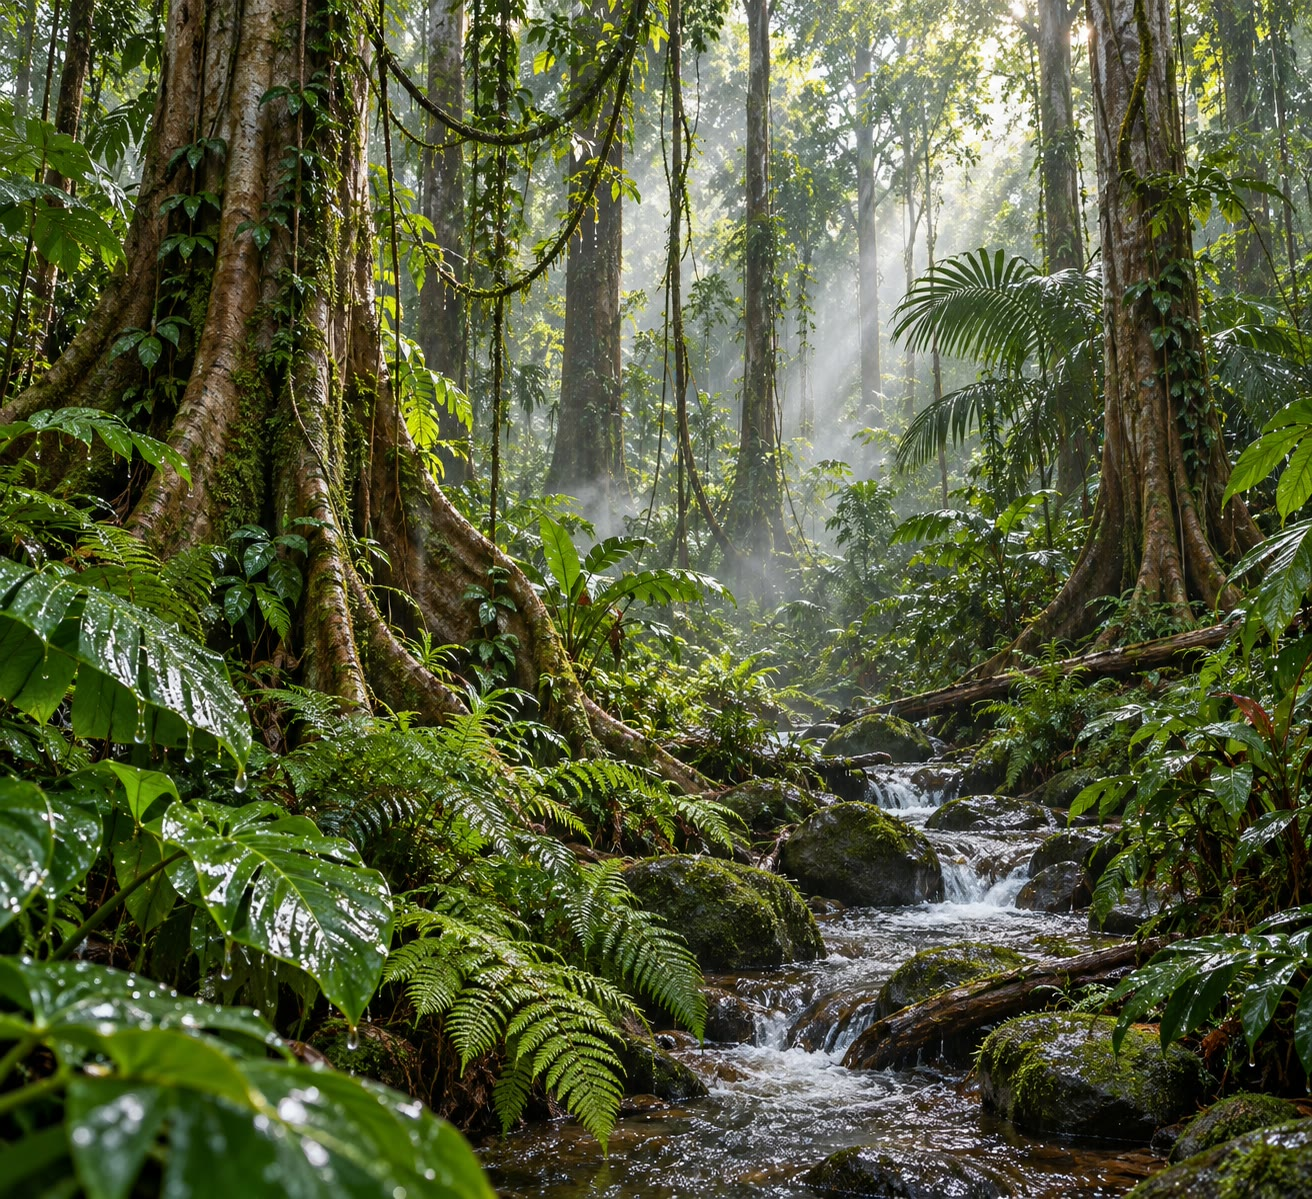
\includegraphics[height=3.6cm]{images/book1/ai/g5-rainforest.jpg}\quad
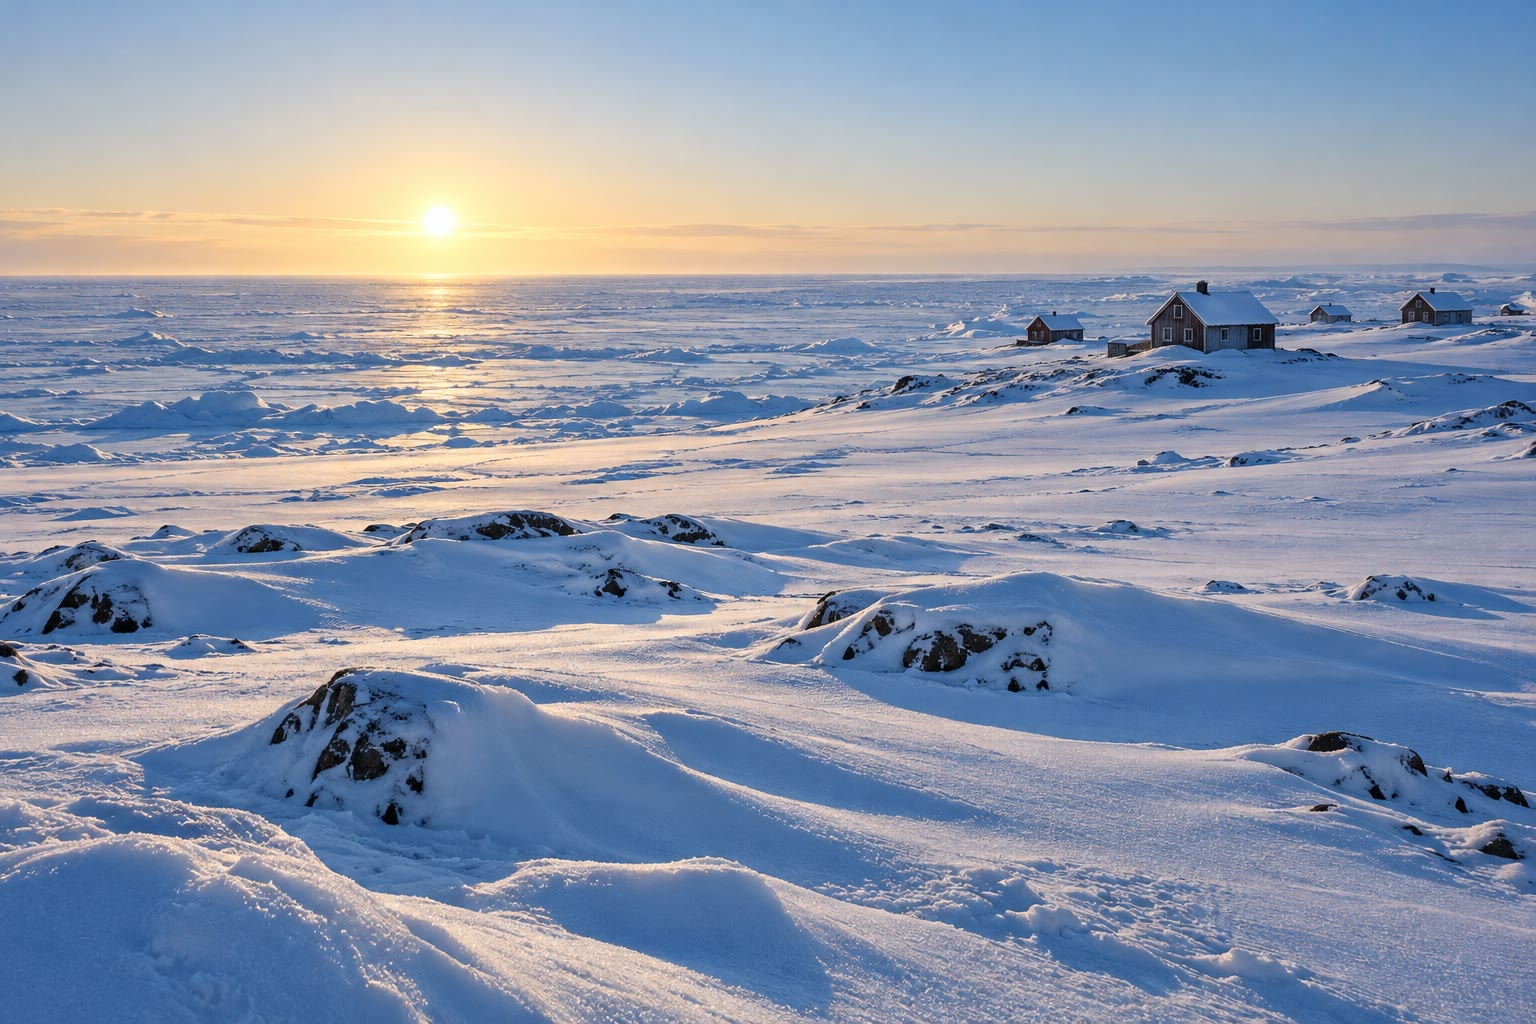
\includegraphics[height=3.6cm]{images/book1/ai/g5-polar-tundra.jpg}

{\small Drie extreme klimaten. Links: de Sonorawoestijn in Arizona, de
\omterm{def:g5:weather-and-climate:desert}{woestijn} van Phoenix, met hoge saguarocactussen en vijgcactussen, die water
opslaan in hun dikke stengels (foto: U.S. National Park Service, Saguaro
National Park, publiek domein). Midden: in een \omterm{def:g5:weather-and-climate:rainforest}{regenwoud} na een bui.
Rechts: een poolkust in de winter, met een bevroren \omterm{def:g2:water-on-earth:ocean}{zee} en een lage Zon
op het middaguur.}
% ledger: nps:sonoran-desert
\end{omfigure}

\paragraph{Het gematigde klimaat.} Seattle zit ertussenin: de lijn stijgt
in de zomer en daalt in de winter, maar nooit erg ver; het regent er flink,
vooral in de herfst en de winter. Dit is een gematigd \omterm{def:g5:weather-and-climate:climate}{klimaat}: geen grote
hitte, geen strenge kou.

\paragraph{Het poolklimaat.} In Utqiaġvik blijft de rode lijn acht maanden
per jaar onder 0~$^\circ$C; in februari is het gemiddelde 24 graden onder
nul. Zelfs in juli, de warmste maand, is het maar ongeveer 5 graden.
% ledger: data:b1-noaa-normals

\section{Warme, gematigde en koude zones}

Waarom is het warm bij de \omterm{def:g3:continents-and-oceans:equator}{evenaar} en koud bij de \omterm{def:g3:continents-and-oceans:poles}{polen}? Door de Zon. Bij de
\omterm{def:g3:continents-and-oceans:equator}{evenaar} staat de middagzon het hele jaar hoog aan de hemel: haar licht
valt bijna recht naar beneden en verwarmt de grond sterk. Bij de \omterm{def:g3:continents-and-oceans:poles}{polen}
blijft de Zon altijd laag: haar licht komt schuin aan, verspreid over een
groot oppervlak, en het verwarmt weinig. In de winter komt de Zon daar
soms helemaal niet op.

Twee paar lijnen rond de \omterm{def:g3:continents-and-oceans:globe}{globe} verdelen de Aarde in \omterm{def:g5:weather-and-climate:climate-zone}{klimaatzones}.

\begin{definition}[Keerkringen en poolcirkels]\label{def:g5:weather-and-climate:tropics}
De twee \emph{keerkringen}\index{keerkring} zijn de lijnen rond de \omterm{def:g3:continents-and-oceans:globe}{globe},
één ten noorden en één ten zuiden van de \omterm{def:g3:continents-and-oceans:equator}{evenaar}, die aangeven hoe ver van
de \omterm{def:g3:continents-and-oceans:equator}{evenaar} de middagzon recht boven je hoofd kan staan: de Kreeftskeerkring
in het noorden, de Steenbokskeerkring in het zuiden. De twee
\emph{poolcirkels}\index{poolcirkel} zijn de lijnen rond de \omterm{def:g3:continents-and-oceans:globe}{globe}, dicht
bij de \omterm{def:g3:continents-and-oceans:poles}{polen}, waarachter de Zon midden in de winter minstens één dag niet
opkomt, en midden in de zomer niet ondergaat: de noordpoolcirkel in het
noorden, de zuidpoolcirkel in het zuiden.
\end{definition}

De schuine stand van de aardas bepaalt waar deze lijnen liggen.

\begin{definition}[Klimaatzones]\label{def:g5:weather-and-climate:climate-zone}
De Aarde is verdeeld in drie soorten \emph{klimaatzones}\index{klimaatzone}:
de \emph{warme zone}, tussen de twee \omterm{def:g5:weather-and-climate:tropics}{keerkringen}, rond de \omterm{def:g3:continents-and-oceans:equator}{evenaar}; de twee
\emph{gematigde zones}, tussen een \omterm{def:g5:weather-and-climate:tropics}{keerkring} en een \omterm{def:g5:weather-and-climate:tropics}{poolcirkel}, waar zomers
en winters verschillen; en de twee \emph{koude zones}, voorbij de
\omterm{def:g5:weather-and-climate:tropics}{poolcirkels}, rond de \omterm{def:g3:continents-and-oceans:poles}{polen}.
\end{definition}

\begin{omfigure}
\begin{tikzpicture}
\begin{axis}[ommap, width=\linewidth, xtick=\empty, ytick=\empty, grid=none,
    axis background/.style={fill=white}, clip=true]
  \addplot[fill=orange!35, draw=none] table {figdata/out/grade-5-climate_zones-hot.dat};
  \addplot[fill=green!20, draw=none] table {figdata/out/grade-5-climate_zones-temperate.dat};
  \addplot[fill=cyan!20, draw=none] table {figdata/out/grade-5-climate_zones-cold.dat};
  \addplot[fill=black!25, fill opacity=0.8, draw=black!60, line width=0.2pt]
    table {figdata/out/shared-geo-land.dat};
  \addplot[black!70, dashed, line width=0.5pt] table {figdata/out/grade-5-climate_zones-lines.dat};
  \draw[black!70, line width=0.6pt] (axis cs:-180,0) -- (axis cs:180,0);
  \addplot[only marks, mark=*, mark size=1.8pt, red!80!black]
    table[x=lon, y=lat] {figdata/out/grade-5-climate_zones-stations.dat};
  \begin{scope}[every node/.style={font=\scriptsize, fill=white, fill opacity=0.75,
      text opacity=1, inner sep=1pt}]
    \node[anchor=west] at (axis cs:-107,33.4) {Phoenix};
    \node[anchor=east] at (axis cs:-158,19.7) {Hilo};
    \node[anchor=west] at (axis cs:-117,47.4) {Seattle};
    \node[anchor=west] at (axis cs:-151,73.5) {Utqiaġvik};
  \end{scope}
  \begin{scope}[every node/.style={font=\scriptsize\bfseries, align=center,
      fill=white, fill opacity=0.7, text opacity=1, inner sep=1pt}]
    \node at (axis cs:-5,83) {koude zone};
    \node at (axis cs:-40,40) {gematigde zone};
    \node at (axis cs:-25,-8) {warme zone};
    \node at (axis cs:95,-45) {gematigde zone};
    \node at (axis cs:-60,-80) {koude zone};
  \end{scope}
\end{axis}
\end{tikzpicture}

{\small De \omterm{def:g5:weather-and-climate:climate-zone}{klimaatzones}. Van boven naar beneden zijn de stippellijnen de
\omterm{def:g5:weather-and-climate:tropics}{noordpoolcirkel}, de \omterm{def:g5:weather-and-climate:tropics}{Kreeftskeerkring}, de \omterm{def:g5:weather-and-climate:tropics}{Steenbokskeerkring} en de
\omterm{def:g5:weather-and-climate:tropics}{zuidpoolcirkel}; de doorgetrokken lijn is de \omterm{def:g3:continents-and-oceans:equator}{evenaar}. De rode stippen zijn
de vier plaatsen van de \omterm{def:g5:weather-and-climate:climate-chart}{klimaatdiagrammen} hierboven.}
% ledger: earth:obliquity, data:b1-noaa-normals
\end{omfigure}

De zones geven een eerste, ruw beeld. Binnen elke zone veranderen veel
andere dingen het \omterm{def:g5:weather-and-climate:climate}{klimaat}: hoe ver een plaats van de \omterm{def:g2:water-on-earth:ocean}{zee} ligt, hoe hoog ze
ligt, waar de wind vandaan komt. Die leer je in de volgende jaren kennen.

\begin{remark}[Phoenix en de zones]\label{rem:g5:weather-and-climate:phoenix}
Op de \omterm{def:g2:drawing-to-map:map}{kaart} van de zones ligt Phoenix iets ten noorden van de
\omterm{def:g5:weather-and-climate:tropics}{Kreeftskeerkring}, in de gematigde zone, en toch is het een hete \omterm{def:g5:weather-and-climate:desert}{woestijn}.
De zones zijn een eerste, ruw beeld: veel van de grote hete \omterm{def:g5:weather-and-climate:desert}{woestijnen}
liggen dicht bij de \omterm{def:g5:weather-and-climate:tropics}{keerkringen}, aan de rand van de warme zone, en in
\cref{ch:g8:winds-global-circulation} leer je waarom.
\end{remark}

\section{Oefeningen}

\begin{exercise}[$\star$]\label{exo:g5:weather-and-climate:1}
\omterm{def:g1:watching-the-weather:weather}{Weer} of \omterm{def:g5:weather-and-climate:climate}{klimaat}?
\begin{enumerate}
  \item[(a)] Vanochtend sneeuwt het in Utqiaġvik.
  \item[(b)] In Phoenix zijn de zomers erg heet en droog.
  \item[(c)] Gistermiddag woei er een harde wind in Seattle.
  \item[(d)] In Hilo regent het elke maand van het jaar veel.
\end{enumerate}
\end{exercise}

\begin{exercise}[$\star$]\label{exo:g5:weather-and-climate:2}
Wat is het \omterm{def:g5:weather-and-climate:climate}{klimaat} van een plaats? Over hoeveel jaar nemen weerkundigen het
gemiddelde van hun metingen om het te beschrijven?
\end{exercise}

\begin{exercise}[$\star$]\label{exo:g5:weather-and-climate:3}
Welke maand is op het \omterm{def:g5:weather-and-climate:climate-chart}{klimaatdiagram} van Seattle de koudste? Welke is de
natste? Komt de temperatuur ooit onder 0~$^\circ$C?
\end{exercise}

\begin{exercise}[$\star$]\label{exo:g5:weather-and-climate:4}
Welke maand is op het \omterm{def:g5:weather-and-climate:climate-chart}{klimaatdiagram} van Utqiaġvik de warmste? Is er een
maand warmer dan 10~$^\circ$C?
\end{exercise}

\begin{exercise}[$\star$]\label{exo:g5:weather-and-climate:5}
In welke \omterm{def:g5:weather-and-climate:climate-zone}{klimaatzone} ligt elk van deze plaatsen: de \omterm{def:g3:continents-and-oceans:equator}{evenaar}; de \omterm{def:g3:continents-and-oceans:poles}{Noordpool};
een plaats halverwege tussen de \omterm{def:g3:continents-and-oceans:equator}{evenaar} en de \omterm{def:g3:continents-and-oceans:poles}{Zuidpool}?
\end{exercise}

\begin{exercise}[$\star$]\label{exo:g5:weather-and-climate:6}
Gebruik de \omterm{def:g2:drawing-to-map:map}{kaart} van de zones. In welke \omterm{def:g5:weather-and-climate:climate-zone}{klimaatzone} ligt elk van de vier
plaatsen: Phoenix, Hilo, Seattle, Utqiaġvik?
\end{exercise}

\begin{exercise}[$\star\star$]\label{exo:g5:weather-and-climate:7}
Hier is de gemiddelde \omterm{def:g4:clouds-rain-snow:precipitation}{regen} van elke maand in Seattle, in millimeter,
afgerond op hele getallen:
\begin{center}
\begin{tabular}{|*{12}{c|}}
\hline
J & F & M & A & M & J & J & A & S & O & N & D\\
\hline
147 & 96 & 106 & 81 & 48 & 37 & 15 & 25 & 41 & 99 & 160 & 145\\
\hline
\end{tabular}
\end{center}
Hoeveel \omterm{def:g4:clouds-rain-snow:precipitation}{regen} valt er in een heel jaar in Seattle? Hoeveel valt er in de
drie maanden december, januari en februari?
% ledger: data:b1-noaa-normals
\end{exercise}

\begin{exercise}[$\star\star$]\label{exo:g5:weather-and-climate:8}
In Phoenix is de gemiddelde temperatuur 14~$^\circ$C in januari en
35~$^\circ$C in juli. In Hilo is ze 22~$^\circ$C in januari en
25~$^\circ$C in juli. Bereken voor elke plaats het verschil tussen juli en
januari. Waar veranderen de seizoenen de temperatuur meer?
% ledger: data:b1-noaa-normals
\end{exercise}

\begin{exercise}[$\star\star$]\label{exo:g5:weather-and-climate:9}
Hier zijn de gemiddelden van een denkbeeldige plaats.
\begin{center}
\begin{tabular}{|l|*{12}{c|}}
\hline
maand & J & F & M & A & M & J & J & A & S & O & N & D\\
\hline
temperatuur ($^\circ$C) & 27 & 27 & 28 & 28 & 28 & 27 & 27 & 27 & 27 & 27 & 27 & 27\\
\hline
\omterm{def:g4:clouds-rain-snow:precipitation}{regen} (mm) & 250 & 230 & 280 & 290 & 260 & 180 & 170 & 160 & 190 & 230 & 250 & 260\\
\hline
\end{tabular}
\end{center}
Is het een woestijn-, een regenwoud-, een gematigd of een poolklimaat? Geef
twee redenen. In welke zone ligt de plaats waarschijnlijk?
\end{exercise}

\begin{exercise}[$\star\star$]\label{exo:g5:weather-and-climate:10}
Denk terug aan de twee ansichtkaarten aan het begin van het hoofdstuk,
verstuurd in dezelfde week van januari. Geef twee verschillende
verklaringen voor hoe kinderen op de ene plek op een zonnig strand kunnen
spelen terwijl anderen op een andere plek een sneeuwpop bouwen.
\end{exercise}

\begin{exercise}[$\star\star\star$]\label{exo:g5:weather-and-climate:11}
Noor zegt: ``Phoenix en Seattle liggen allebei in de gematigde zone, dus ze
moeten hetzelfde \omterm{def:g5:weather-and-climate:climate}{klimaat} hebben.'' Laat met de \omterm{def:g5:weather-and-climate:climate-chart}{klimaatdiagrammen} zien dat
ze ongelijk heeft: vergelijk hun temperaturen en hun \omterm{def:g4:clouds-rain-snow:precipitation}{regen}. Zeg daarna wat
de \omterm{def:g5:weather-and-climate:climate-zone}{klimaatzones} ons vertellen, en wat niet.
\end{exercise}
